%% abtex2-modelo-artigo.tex, v-1.9.7 laurocesar
%% Copyright 2012-2018 by abnTeX2 group at http://www.abntex.net.br/ 
%%
%% This work may be distributed and/or modified under the
%% conditions of the LaTeX Project Public License, either version 1.3
%% of this license or (at your option) any later version.
%% The latest version of this license is in
%%   http://www.latex-project.org/lppl.txt
%% and version 1.3 or later is part of all distributions of LaTeX
%% version 2005/12/01 or later.
%%
%% This work has the LPPL maintenance status `maintained'.
%% 
%% The Current Maintainer of this work is the abnTeX2 team, led
%% by Lauro César Araujo. Further information are available on 
%% http://www.abntex.net.br/
%%
%% This work consists of the files abntex2-modelo-artigo.tex and
%% abntex2-modelo-references.bib
%%
% ---------------------------------------------------------------
% ---------------------------------------------------------------
% abnTeX2: Modelo de Artigo Acadêmico em conformidade com
% ABNT NBR 6022:2018: Informação e documentação - Artigo em publicação 
% periódica científica - Apresentação
% ---------------------------------------------------------------
% Adaptado para uso na instituição acadêmica Senai Cimatec.
% 25/05/2022
% -----------------------------------------------------------------

\documentclass[
	% -- opções da classe memoir --
	article,			% indica que é um artigo acadêmico
	11pt,				% tamanho da fonte
	oneside,			% para impressão apenas no recto. Oposto a twoside
	a4paper,			% tamanho do papel. 
	% -- opções da classe abntex2 --
	%chapter=TITLE,		% títulos de capítulos convertidos em letras maiúsculas
	%section=TITLE,		% títulos de seções convertidos em letras maiúsculas
	%subsection=TITLE,	% títulos de subseções convertidos em letras maiúsculas
	%subsubsection=TITLE % títulos de subsubseções convertidos em letras maiúsculas
	% -- opções do pacote babel --
	english,			% idioma adicional para hifenização
	brazil,				% o último idioma é o principal do documento
	sumario=tradicional
	]{abntex2}

% --- Pacotes fundamentais 
\usepackage{lmodern}		% Usa a fonte Latin Modern
\usepackage[T1]{fontenc}	% Selecao de codigos de fonte.
\usepackage[utf8]{inputenc}	% Conversão automática dos acentos
\usepackage{indentfirst}	% Indenta o 1. parágrafo de cada seção.
\usepackage{nomencl} 		% Lista de simbolos
\usepackage{color}			% Controle das cores
\usepackage{xcolor}         % Criação de label com cores específicas
\usepackage{graphicx}		% Inclusão de gráficos
\usepackage{microtype} 		% para melhorias de justificação
% --- Pacotes extras
\usepackage{lipsum}			% para geração de dummy text
% --- Pacotes de citações
\usepackage[brazilian,hyperpageref]{backref}	
\usepackage[alf]{abntex2cite}

\usepackage{tikz} % Pacotes para manipulação de imagens
\usepackage{float} % habilita a opção [H] (here) nas imagens
\usepackage{listings} % inserção de código no PDF

% ---
% Configurações do pacote listings

% criação de cores personalizadas
\definecolor{gray}{RGB}{160, 161, 167}
\definecolor{yellow}{RGB}{197, 163, 50}
\definecolor{backcolour}{RGB}{249, 249, 249}
\definecolor{blu}{RGB}{0, 152, 221}

% configurações de estilo personalizado para o pacote listing
\lstdefinestyle{bluloco-light}{
    backgroundcolor=\color{backcolour},   
    commentstyle=\itshape\color{gray},
    keywordstyle=\bfseries\color{blu},
    numberstyle=\tiny\color{gray},
    stringstyle=\color{yellow},
    basicstyle=\ttfamily\footnotesize,
    breakatwhitespace=false,
    breaklines=true,                 
    captionpos=b,                    
    keepspaces=true,                 
    numbers=left,                    
    numbersep=5pt,                  
    showspaces=false,                
    showstringspaces=false,
    showtabs=false,                  
    tabsize=2
}

% definição do estilo do pacote listing
\lstset{style=bluloco-light}

%//todo o que quem dizer isso? porque? é necessário fazer comentários.
%//valar erick suzart
%//checked mhar-vell OK

% mapeamento de caracteres especiais: necessário para adicionar caracteres
% especiais em código utilizando o pacote listing
\lstset{literate=
  {á}{{\'a}}1 {é}{{\'e}}1 {í}{{\'i}}1 {ó}{{\'o}}1 {ú}{{\'u}}1
  {Á}{{\'A}}1 {É}{{\'E}}1 {Í}{{\'I}}1 {Ó}{{\'O}}1 {Ú}{{\'U}}1
  {à}{{\`a}}1 {è}{{\`e}}1 {ì}{{\`i}}1 {ò}{{\`o}}1 {ù}{{\`u}}1
  {À}{{\`A}}1 {È}{{\'E}}1 {Ì}{{\`I}}1 {Ò}{{\`O}}1 {Ù}{{\`U}}1
  {ä}{{\"a}}1 {ë}{{\"e}}1 {ï}{{\"i}}1 {ö}{{\"o}}1 {ü}{{\"u}}1
  {Ä}{{\"A}}1 {Ë}{{\"E}}1 {Ï}{{\"I}}1 {Ö}{{\"O}}1 {Ü}{{\"U}}1
  {â}{{\^a}}1 {ê}{{\^e}}1 {î}{{\^i}}1 {ô}{{\^o}}1 {û}{{\^u}}1
  {Â}{{\^A}}1 {Ê}{{\^E}}1 {Î}{{\^I}}1 {Ô}{{\^O}}1 {Û}{{\^U}}1
  {ã}{{\~a}}1 {ẽ}{{\~e}}1 {ĩ}{{\~i}}1 {õ}{{\~o}}1 {ũ}{{\~u}}1
  {Ã}{{\~A}}1 {Ẽ}{{\~E}}1 {Ĩ}{{\~I}}1 {Õ}{{\~O}}1 {Ũ}{{\~U}}1
  {œ}{{\oe}}1 {Œ}{{\OE}}1 {æ}{{\ae}}1 {Æ}{{\AE}}1 {ß}{{\ss}}1
  {ű}{{\H{u}}}1 {Ű}{{\H{U}}}1 {ő}{{\H{o}}}1 {Ő}{{\H{O}}}1
  {ç}{{\c c}}1 {Ç}{{\c C}}1 {ø}{{\o}}1 {å}{{\r a}}1 {Å}{{\r A}}1
  {€}{{\euro}}1 {£}{{\pounds}}1 {«}{{\guillemotleft}}1
  {»}{{\guillemotright}}1 {ñ}{{\~n}}1 {Ñ}{{\~N}}1 {¿}{{?`}}1
}

% ---
% Configurações do pacote backref
% Usado sem a opção hyperpageref de backref
\renewcommand{\backrefpagesname}{Citado na(s) página(s):~}
\renewcommand{\backref}{}
\renewcommand*{\backrefalt}[4]{
	\ifcase #1 %
		Nenhuma citação no texto.%
	\or
		Citado na página #2.%
	\else
		Citado #1 vezes nas páginas #2.%
	\fi}%

% ........................................................................
% CONFIGURAÇÃO DO ENDEREÇO DAS FIGURAS
\graphicspath{{source/pictures/}}

% --- Informações de dados para CAPA e FOLHA DE ROSTO ---
\titulo{Construção de plataforma de jogo em Processing com integração de Arduino.}
\tituloestrangeiro{}
\autor{
      Ludmila Nascimento Dos Anjos
      \\[0.5cm] 
      Rafael Ferreira Viana de Mello
      \\[0.5cm] 
      Kauan Dantas Brito da Silva
      \\[0.5cm] 
      Gabriel Lopes Guimarães
      }
\local{Brasil}
\data{20/06/2022}
% ---
\definecolor{blue}{RGB}{41,5,195}
% --- informações do PDF
\makeatletter
\hypersetup{
     	%pagebackref=true,
		pdftitle={\@title}, 
		pdfauthor={\@author},
    	pdfsubject={Modelo de artigo científico com abnTeX2},
	    pdfcreator={LaTeX with abnTeX2},
		pdfkeywords={abnt}{latex}{abntex}{abntex2}{atigo científico}, 
		colorlinks=true,  % false: boxed links; true: colored links
    	linkcolor=blue,   % color of internal links
    	citecolor=blue,   % color of links to bibliography
    	filecolor=magenta,% color of file links
		urlcolor=blue,
		bookmarksdepth=4
}
\makeatother
\makeindex
\setlrmarginsandblock{3cm}{3cm}{*}
\setulmarginsandblock{3cm}{3cm}{*}
\checkandfixthelayout
% ---
\setlength{\parindent}{1.3cm}
\setlength{\parskip}{0.2cm}  
\SingleSpacing
% ----
\begin{document}
\selectlanguage{brazil}
\frenchspacing
% ----------------------------------------------------------
% ELEMENTOS PRÉ-TEXTUAIS
% ----------------------------------------------------------
% Se desejar escrever o artigo em duas colunas, descomente a linha abaixo e a linha com o texto ``FIM DE ARTIGO EM DUAS COLUNAS''.
% \twocolumn[    		% INICIO DE ARTIGO EM DUAS COLUNAS
%
% página de titulo principal (obrigatório)
\maketitle
% titulo em outro idioma (opcional)

% resumo em português
\begin{resumoumacoluna}
   Conforme a ABNT NBR 6022:2018, o resumo no idioma do documento é elemento obrigatório.
   Constituído de uma sequência de frases concisas e objetivas e não de uma simples enumeração de tópicos, não ultrapassando 250 palavras, seguido, logo abaixo, das palavras representativas do conteúdo do trabalho, isto é palavras-chave e/ou descritores, conforme a NBR 6028. (\ldots)
   As palavras-chave devem figurar logo abaixo do resumo, antecedidas da expressão Palavras-chave:, separadas entre si por ponto e finalizadas também por ponto.

   \vspace{\onelineskip}

   \noindent
   \textbf{Palavras-chave}: latex. abntex. editoração de texto.
\end{resumoumacoluna}

% resumo em inglês
\renewcommand{\resumoname}{Abstract}
\begin{resumoumacoluna}
   \begin{otherlanguage*}{english}
      According to ABNT NBR 6022:2018, an abstract in foreign language is optional.

      \vspace{\onelineskip}

      \noindent
      \textbf{Keywords}: latex. abntex.
   \end{otherlanguage*}
\end{resumoumacoluna}

% ]  				% FIM DE ARTIGO EM DUAS COLUNAS
% ----------------------------------------------------------
% ELEMENTOS TEXTUAIS
% ----------------------------------------------------------
\textual
%
\section{Introdução}

Em 1972, na garagem de um grupo de engenheiros que criariam uma empresa de jogos futuramente, a Atari, surgiu, de um pequeno exercício de simulação o que muitos consideram como o primeiro jogo da história: o "Pong". Na tentativa de simular uma partida de tênis de mesa ou "Ping-Pong" como é conhecido, o jogo eletrônico foi incrementado pelo grupo que tornou o jogo mais divertido e apropriado para o público.

	Apesar de ter sido recusado por um cliente, alegando que prefereria um jogo de carros, um dos criadores não desistiu. "Bushnell convenceu um bar, chamado Andy Capp's, em Sunnyvale, na Califórnia, a instalar o Pong em uma máquina de fliperama —daquelas que funcionam com a inserção de moedas" (UOL, 2022). 

	Esse foi o salto inicial que, não só impulsionou o sucesso do jogo "Pong", mas também do mundo dos fliperamas, que teve sua alta na década de 80.

	Com isso em mente, o presente trabalho tem como finalidade de recriar o jogo "Pong" utilizando de tecnologias mais modernas. Em suma, através da integração de um Arduino UNO, que irá receber a informação dos botões e joysticks(potênciometros) e enviará por comunicação serial ao jogo, desenvolvido utilizando a linguagem de programação Open Source "Processing", utilizada para programação dentro do contexto de artes visuais[2].


\section{Desenvolvimento}


\section{Materiais e Métodos}

Para o desenvolvimento do presente projeto, os componentes serão separados em duas partes: Hardware e Software.
	A parte referente ao hardware tangencia o físico do projeto, ou seja, os componentes eletrônicos e os controles. Já o Software refere-se à "mente do dispositivo", o que estará disposto na forma de programação, que será o próprio jogo. Assim sendo, os componentes são divididos da seguinte forma:
	
\subsection{Hardware}
\begin{itemize}
\item Fios conectores;
\item 3 Resistores de 1K$\Omega$, para proteger os botões. 
\item 2 Botões com capa branca;
\item 2 Potenciômetros, que funcionarão como os joysticks;
\item 2 cases impressas em 3D, que funcionará como os controles do jogo;
\item 1 Arduino UNO R3, que coletará as informações dos botões e potênciometros;
\item 1 Computador; \vspace*{0.5cm}
\end{itemize}

\subsection{Software}
\begin{itemize}
\item Visual Studio Code;
\item GitHub, como plataforma para hospedar o desenvolvimento;
\item TinkerCad(C), para simular o hardware do jogo;
\item Processing; 
\end{itemize}
%*----------- SLIDE -------------------------------------------------------------
\begin{frame}[t]{Hardware}

	\begin{itemize}
        \item Circuito utilizado como os controles do jogo
	\item Os potenciômetros controlam as barras (paddles)
	\item Os botões fazem a transição de telas e pausam o jogo.
    \end{itemize}
   
	\vspace{0.3cm}
	\begin{columns}
		% Column 1
		\begin{column}{0.5\textwidth}
			\begin{figure}
				\centering
					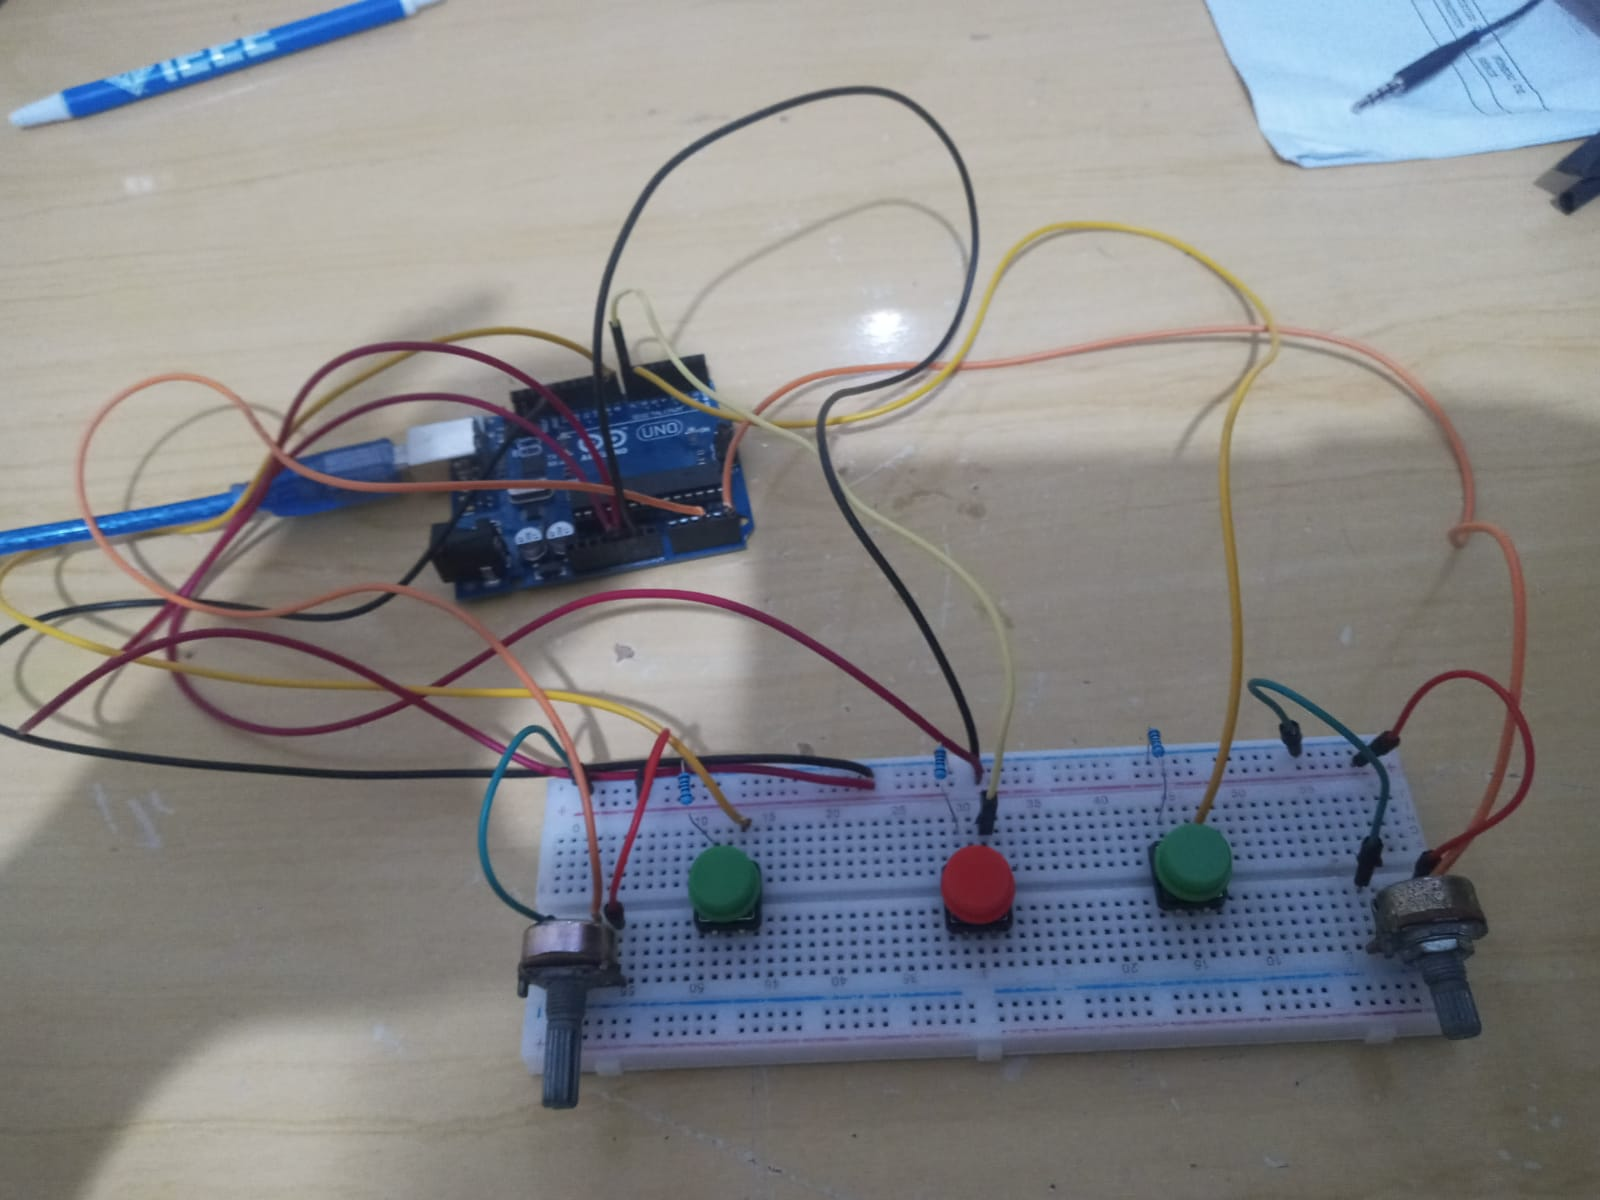
\includegraphics[width=0.6\textwidth]{circuito}
			\end{figure}
		\end{column}
			% Column 2    
			\begin{column}{0.7\textwidth}
				\begin{figure}
					\centering
						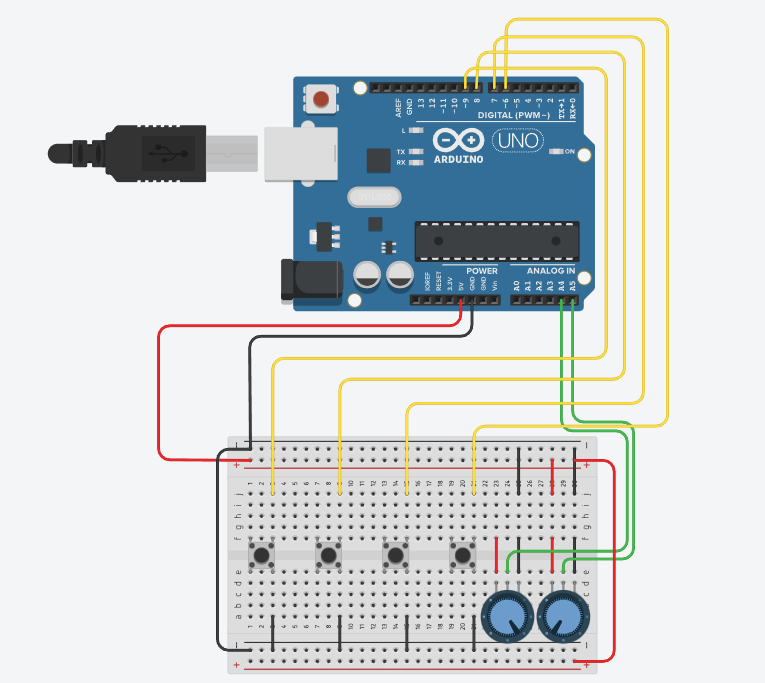
\includegraphics[width=0.4\textwidth]{esquematico-arduino}
				\end{figure}
			\end{column}
		\end{columns}

%*----------- notes
    \note[item]{Notes can help you to remember important information. Turn on the notes option.}
\end{frame}
%-
%*----------- SLIDE -------------------------------------------------------------
\begin{frame}[c]{Hardware - Controles}
 
  \begin{itemize}
      \item Modelos Impressos 3D para acomodar os botões e potenciômetros do circuito.
	\item Estes também são mais cômodos para os jogadores
    \end{itemize}
\vspace{0.3cm}
\begin{columns}
	% Column 1
	\begin{column}{0.4\textwidth}
		\begin{figure}
			\centering
    			\includegraphics[width=0.6\textwidth]{botão}
    			\caption{Os modelos impressos.}
    			%%\label{fig:question}
		\end{figure}
	\end{column}
		% Column 2    
		\begin{column}{0.4\textwidth}
			\begin{figure}
				\centering
    				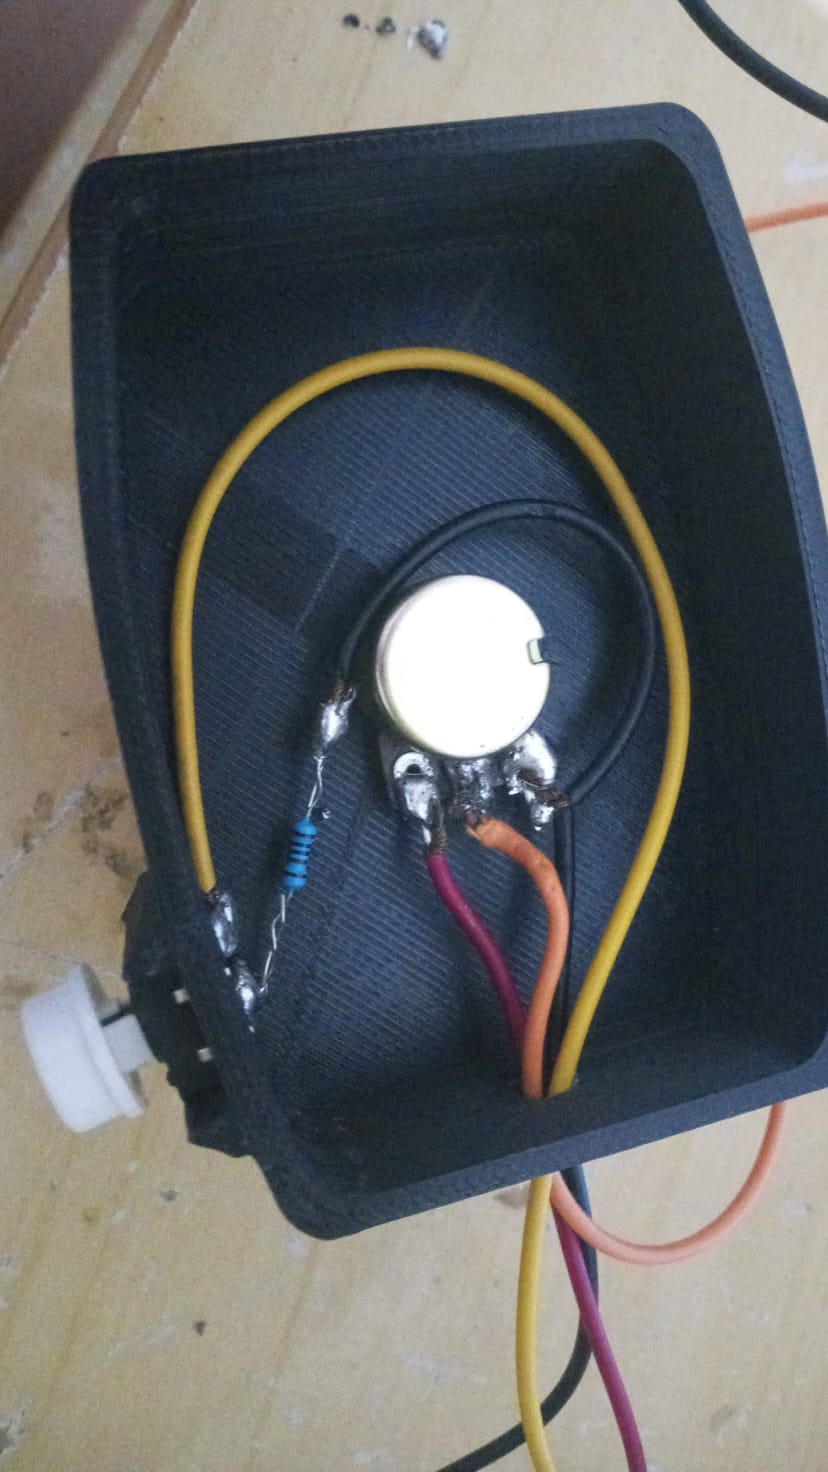
\includegraphics[width=0.4\textwidth]{solda}
    				\caption{A solda cos componentes no controle.}
    				%%\label{fig:question}
			\end{figure}
		\end{column}
	\end{columns}
%*----------- notes
    \note[item]{Notes can help you to remember important information. Turn on the notes option.}
 \end{frame}
%-
%*----------- SLIDE -------------------------------------------------------------
\begin{frame}[fragile]{Hardware - Arduino}
	 
\scriptsize
\begin{columns}
% Column 1
\begin{column}{0.5\textwidth}
	\begin{lstlisting}[language=C]
const int pot1 = A0, pot2 = A1; 
const int b01 = 8, b02 = 7; 
int v_pot1 = 0, v_pot2 = 0; 
bool v_b01,v_b02; 
int arr[10];

void setup() {
	Serial.begin(9600);
	pinMode(pot1, INPUT);
	pinMode(pot2, INPUT);
	for(int i = 7; i <= 8; i++){
	pinMode(i, INPUT_PULLUP);
	}
}
	\end{lstlisting}
\end{column}
% Column 2    
\begin{column}{0.55\textwidth}
	\begin{lstlisting}[language=C]
void loop() {

v_pot1 = map(analogRead(pot1),0,1023,0,255);
Serial.print(String(v_pot1) + "-");

v_pot2 = map(analogRead(pot2),0,1023,0,255);
Serial.print(String(v_pot2) + "-");

v_b01 = !digitalRead(b01);
v_b02 = !digitalRead(b02);

Serial.print(String(v_b01) + "-");
Serial.print(String(v_b02) + "\n");
delay(50);

}		
	\end{lstlisting}
\end{column}
\end{columns} 


%*----------- notes
    \note[item]{Notes can help you to remember important information. Turn on the notes option.}
 \end{frame}
%-
%*----------- SLIDE -------------------------------------------------------------
\begin{frame}[c]{Hardware - Arduino}
\vspace{0.2cm}
\begin{itemize}
        \item Como pode ser visto, uma string de modelo [x-x-x-x] é enviada ao Processing serialmente.
	  \item No Processing, essa string será separada em caracteres e cada um sera atribuido a sua respectiva classe.
    \end{itemize}

\begin{figure}
	\centering
    	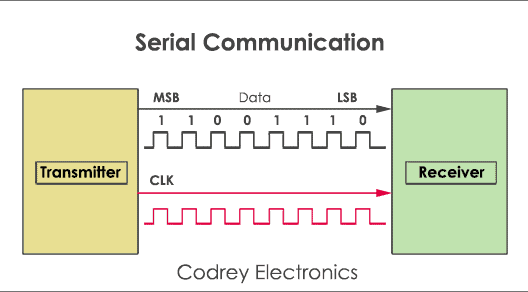
\includegraphics[width=0.4\textwidth]{serial}
    	%\caption{Representação d}
    	%%\label{fig:question}
\end{figure}

%*----------- notes
    \note[item]{Notes can help you to remember important information. Turn on the notes option.}
 \end{frame}
 %-
%*----------- SLIDE -------------------------------------------------------------
\begin{frame}
    

    
%*----------- notes
    \note[item]{Notes can help you to remember important information. Turn on the notes option.}
 \end{frame}
 %-
%*----------- SLIDE -------------------------------------------------------------
\begin{frame}
    %\transdissolve[duration=0.5]
    %\hspace*{-1cm}

  
 %*----------- notes__
    \note[item]{Notes can help you to remember important information. Turn on the notes option.}
\end{frame}
%-
%*----------- SLIDE -------------------------------------------------------------
\begin{frame}
    
  
 %*----------- notes__
    \note[item]{Notes can help you to remember important information. Turn on the notes option.}
\end{frame}
%-
%*----------- SLIDE -------------------------------------------------------------
\begin{frame}
    %\transdissolve[duration=0.5]
    
  
 %*----------- notes__
    \note[item]{Notes can help you to remember important information. Turn on the notes option.}
\end{frame}
%-
%*----------- SLIDE -------------------------------------------------------------
\begin{frame}
    %\transdissolve[duration=0.5]
    %\hspace*{-1cm}

  
 %*----------- notes
    \note[item]{Notes can help you to remember important information. Turn on the notes option.}
\end{frame}
 %-
%*----------- SLIDE -------------------------------------------------------------
\begin{frame}
    %\transdissolve[duration=0.5]
    %\hspace*{-1cm}
    
  
 %*----------- notes
    \note[item]{Notes can help you to remember important information. Turn on the notes option.}
\end{frame}
%-


\section{Conclusão}

\lipsum[1]

\begin{citacao}
    \lipsum[2]
\end{citacao}

\lipsum[3]
% ----------------------------------------------------------
\bookmarksetup{startatroot}% Finaliza a parte no bookmark do PDF, para que se inicie o bookmark na raiz 
% ----------------------------------------------------------
% ELEMENTOS PÓS-TEXTUAIS
% ----------------------------------------------------------
\postextual
% 
% Referências bibliográficas
% ----------------------------------------------------------
\bibliography{references}
% 
% Agradecimentos
% ----------------------------------------------------------
\section*{Agradecimentos}
Texto sucinto aprovado pelo periódico em que será publicado. Último elemento pós-textual.
%
\end{document}
